\documentclass[tikz,border=8pt]{standalone}
% Shared look for every TikZ diagram. Load with % Shared look for every TikZ diagram. Load with % Shared look for every TikZ diagram. Load with \input{../../tools/tikz-style.tex}
\usepackage[T1]{fontenc}
\usepackage{lmodern}
\renewcommand{\sfdefault}{lmr}  % diagrams use the same serif as the text
\usetikzlibrary{arrows.meta, positioning, shapes.geometric, calc, fit, backgrounds}
\definecolor{cblue}{HTML}{4C78A8}
\definecolor{corange}{HTML}{F58518}
\definecolor{cgreen}{HTML}{54A24B}
\definecolor{cred}{HTML}{E45756}
\definecolor{cpurple}{HTML}{B279A2}
\definecolor{cgrey}{HTML}{6B6B6B}
\tikzset{
  every picture/.style={font=\sffamily, line width=1.2pt},
  box/.style={draw=#1, fill=#1!12, rounded corners=4pt, align=center, inner sep=7pt, minimum height=1.1cm},
  box/.default=cgrey,
  arrow/.style={-{Stealth[length=3mm]}, draw=cgrey, line width=1.4pt},
  title/.style={font=\sffamily\bfseries\Large},
  note/.style={font=\sffamily\small, text=cgrey, align=center},
}
\AtBeginDocument{\hyphenpenalty=10000 \exhyphenpenalty=10000}

\usepackage[T1]{fontenc}
\usepackage{lmodern}
\renewcommand{\sfdefault}{lmr}  % diagrams use the same serif as the text
\usetikzlibrary{arrows.meta, positioning, shapes.geometric, calc, fit, backgrounds}
\definecolor{cblue}{HTML}{4C78A8}
\definecolor{corange}{HTML}{F58518}
\definecolor{cgreen}{HTML}{54A24B}
\definecolor{cred}{HTML}{E45756}
\definecolor{cpurple}{HTML}{B279A2}
\definecolor{cgrey}{HTML}{6B6B6B}
\tikzset{
  every picture/.style={font=\sffamily, line width=1.2pt},
  box/.style={draw=#1, fill=#1!12, rounded corners=4pt, align=center, inner sep=7pt, minimum height=1.1cm},
  box/.default=cgrey,
  arrow/.style={-{Stealth[length=3mm]}, draw=cgrey, line width=1.4pt},
  title/.style={font=\sffamily\bfseries\Large},
  note/.style={font=\sffamily\small, text=cgrey, align=center},
}
\AtBeginDocument{\hyphenpenalty=10000 \exhyphenpenalty=10000}

\usepackage[T1]{fontenc}
\usepackage{lmodern}
\renewcommand{\sfdefault}{lmr}  % diagrams use the same serif as the text
\usetikzlibrary{arrows.meta, positioning, shapes.geometric, calc, fit, backgrounds}
\definecolor{cblue}{HTML}{4C78A8}
\definecolor{corange}{HTML}{F58518}
\definecolor{cgreen}{HTML}{54A24B}
\definecolor{cred}{HTML}{E45756}
\definecolor{cpurple}{HTML}{B279A2}
\definecolor{cgrey}{HTML}{6B6B6B}
\tikzset{
  every picture/.style={font=\sffamily, line width=1.2pt},
  box/.style={draw=#1, fill=#1!12, rounded corners=4pt, align=center, inner sep=7pt, minimum height=1.1cm},
  box/.default=cgrey,
  arrow/.style={-{Stealth[length=3mm]}, draw=cgrey, line width=1.4pt},
  title/.style={font=\sffamily\bfseries\Large},
  note/.style={font=\sffamily\small, text=cgrey, align=center},
}
\AtBeginDocument{\hyphenpenalty=10000 \exhyphenpenalty=10000}

\begin{document}
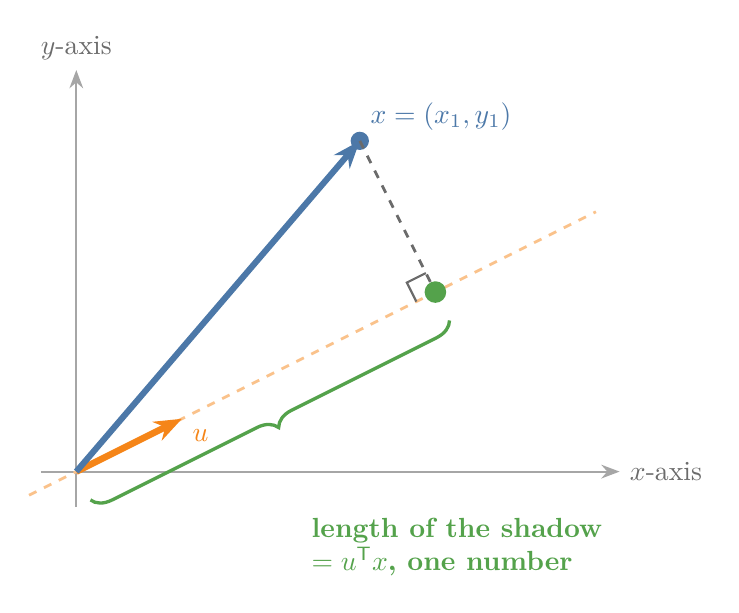
\begin{tikzpicture}[scale=1.5]
  \draw[cgrey!60, line width=0.8pt, -{Stealth}] (-0.3,0) -- (4.6,0) node[right, text=cgrey] {$x$-axis};
  \draw[cgrey!60, line width=0.8pt, -{Stealth}] (0,-0.3) -- (0,3.4) node[above, text=cgrey] {$y$-axis};
  % direction line through the origin
  \draw[corange!50, line width=1pt, dashed] (-0.4,-0.2) -- (4.4,2.2);
  % unit vector u
  \draw[corange, line width=2.4pt, -{Stealth[length=3.5mm]}] (0,0) -- ({2/sqrt(5)},{1/sqrt(5)}) node[below right=-1pt, font=\bfseries, text=corange] {$u$};
  % the point x
  \coordinate (X) at (2.4,2.8);
  \draw[cblue, line width=2.2pt, -{Stealth[length=3.5mm]}] (0,0) -- (X);
  \fill[cblue] (X) circle (2.2pt) node[above right, text=cblue, font=\bfseries] {$x = (x_1, y_1)$};
  % its projection: (u.x) u with u=(2,1)/sqrt5 -> u.x = (4.8+2.8)/sqrt5 ; foot = (u.x)*u = (7.6/5)*(2,1)
  \coordinate (P) at (3.04,1.52);
  \draw[cgrey, dashed, line width=1pt] (X) -- (P);
  \draw[cgrey, line width=0.8pt] ($(P)!0.18cm!(X)$) -- ($($(P)!0.18cm!(X)$)!0.18cm!90:(X)$) -- ($(P)!0.18cm!(0,0)$);
  \fill[cgreen] (P) circle (2.6pt);
  \draw[decorate, decoration={brace, amplitude=7pt, mirror}, draw=cgreen, line width=1.2pt]
    (0.12,-0.24) -- (3.16,1.28);
  \node[text=cgreen, font=\bfseries, align=left, anchor=north west] at (1.9,-0.3) {length of the shadow\\$= u^{\mathsf T}x$, one number};
\end{tikzpicture}
\end{document}
